\documentclass[]{article}
\usepackage{lmodern}
\usepackage{amssymb,amsmath}
\usepackage{ifxetex,ifluatex}
\usepackage{fixltx2e} % provides \textsubscript
\ifnum 0\ifxetex 1\fi\ifluatex 1\fi=0 % if pdftex
  \usepackage[T1]{fontenc}
  \usepackage[utf8]{inputenc}
\else % if luatex or xelatex
  \ifxetex
    \usepackage{mathspec}
  \else
    \usepackage{fontspec}
  \fi
  \defaultfontfeatures{Ligatures=TeX,Scale=MatchLowercase}
\fi
% use upquote if available, for straight quotes in verbatim environments
\IfFileExists{upquote.sty}{\usepackage{upquote}}{}
% use microtype if available
\IfFileExists{microtype.sty}{%
\usepackage{microtype}
\UseMicrotypeSet[protrusion]{basicmath} % disable protrusion for tt fonts
}{}
\usepackage[margin=1in]{geometry}
\usepackage{hyperref}
\hypersetup{unicode=true,
            pdftitle={Análise 1},
            pdfauthor={Raul de Sá Durlo},
            pdfborder={0 0 0},
            breaklinks=true}
\urlstyle{same}  % don't use monospace font for urls
\usepackage{graphicx,grffile}
\makeatletter
\def\maxwidth{\ifdim\Gin@nat@width>\linewidth\linewidth\else\Gin@nat@width\fi}
\def\maxheight{\ifdim\Gin@nat@height>\textheight\textheight\else\Gin@nat@height\fi}
\makeatother
% Scale images if necessary, so that they will not overflow the page
% margins by default, and it is still possible to overwrite the defaults
% using explicit options in \includegraphics[width, height, ...]{}
\setkeys{Gin}{width=\maxwidth,height=\maxheight,keepaspectratio}
\usepackage[normalem]{ulem}
% avoid problems with \sout in headers with hyperref:
\pdfstringdefDisableCommands{\renewcommand{\sout}{}}
\IfFileExists{parskip.sty}{%
\usepackage{parskip}
}{% else
\setlength{\parindent}{0pt}
\setlength{\parskip}{6pt plus 2pt minus 1pt}
}
\setlength{\emergencystretch}{3em}  % prevent overfull lines
\providecommand{\tightlist}{%
  \setlength{\itemsep}{0pt}\setlength{\parskip}{0pt}}
\setcounter{secnumdepth}{5}
% Redefines (sub)paragraphs to behave more like sections
\ifx\paragraph\undefined\else
\let\oldparagraph\paragraph
\renewcommand{\paragraph}[1]{\oldparagraph{#1}\mbox{}}
\fi
\ifx\subparagraph\undefined\else
\let\oldsubparagraph\subparagraph
\renewcommand{\subparagraph}[1]{\oldsubparagraph{#1}\mbox{}}
\fi

%%% Use protect on footnotes to avoid problems with footnotes in titles
\let\rmarkdownfootnote\footnote%
\def\footnote{\protect\rmarkdownfootnote}

%%% Change title format to be more compact
\usepackage{titling}

% Create subtitle command for use in maketitle
\newcommand{\subtitle}[1]{
  \posttitle{
    \begin{center}\large#1\end{center}
    }
}

\setlength{\droptitle}{-2em}
  \title{Análise 1}
  \pretitle{\vspace{\droptitle}\centering\huge}
  \posttitle{\par}
\subtitle{\emph{Homicídios por 100mil habitantes - Estado de São paulo (2000 -
2010)}}
  \author{Raul de Sá Durlo\footnote{Mestre em Economia - Unesp/FCLAr}}
  \preauthor{\centering\large\emph}
  \postauthor{\par}
  \predate{\centering\large\emph}
  \postdate{\par}
  \date{12 setembro 2017}


\begin{document}
\maketitle
\begin{abstract}
Esta seção tem como objetivo comparar a evolução da criminalidade no
município de São Paulo com as demais regiões do Estado de São Paulo.
Para isso, os municípios do estado de São Paulo são divididos em três
grandes grupos (Interior, Região Metropolitana de São Paulo e Capital).
Os crimes analisados são homocídios, roubo de veículo e furto de
veículo.
\end{abstract}

\subsection{Introdução}\label{introducao}

Neste \sout{breve} artigo, foi explorada a evolução das taxas de
homicídio, de roubo de veículos e furtos de veículos no Estado de São
Paulo, que por sua vez foi dividido em três grandes grupos: Capital,
Interior, e Grande São Paulo.

O município de São Paulo é destacado em relação aos demais municípios do
estado para justificar sua escolha para análise em relação aos demais.

\subsection{Metodologia}\label{metodologia}

Os dados referem-se ao número de ocorrências registradas entre os anos
de 2000 e 2010 para cada um dos crimes citados. Como sua interpretação é
sensível à mudanças demográficas, os dados foram normalizados em relação
à população residente, sendo calculado, portanto, uma taxa de homicídios
por 100.000 habitantes:

\[\left(\frac{crime_i}{população_i}\right)100000\]

Os dados de ocorrências criminais são provenientes das Estatísticas
Trimestrais\footnote{\url{http://www.ssp.sp.gov.br/estatistica/trimestrais.aspx}}
da Secretaria Estadual de Segurança Pública do Estado de São Paulo. Já
os dados da população residente foram extraídos das Estimativas
utilizadas pelo Tribunal de Contas da União para determinação das cotas
do Fundo de Participação dos Municípios\footnote{\url{http://tabnet.datasus.gov.br/cgi/deftohtm.exe?ibge/cnv/poptsp.def}}(\url{http://tabnet.datasus.gov.br/cgi/deftohtm.exe?ibge/cnv/poptsp.def}).

\subsection{Resultados}\label{resultados}

\begin{table}[!htbp] \centering 
  \caption{Estatísticas descritivas - Capital} 
  \label{} 
\begin{tabular}{@{\extracolsep{5pt}}lccccc} 
\\[-1.8ex]\hline 
\hline \\[-1.8ex] 
Statistic & \multicolumn{1}{c}{N} & \multicolumn{1}{c}{Mean} & \multicolumn{1}{c}{St. Dev.} & \multicolumn{1}{c}{Min} & \multicolumn{1}{c}{Max} \\ 
\hline \\[-1.8ex] 
tx\_homicidio & 11 & 27.76 & 16.32 & 10.64 & 53.22 \\ 
tx\_furto & 11 & 474.90 & 74.07 & 381.94 & 605.90 \\ 
tx\_roubo & 11 & 392.81 & 95.54 & 286.95 & 614.81 \\ 
\hline \\[-1.8ex] 
\end{tabular} 
\end{table}

\begin{table}[!htbp] \centering 
  \caption{Estatísticas descritivas - Grande SP} 
  \label{} 
\begin{tabular}{@{\extracolsep{5pt}}lccccc} 
\\[-1.8ex]\hline 
\hline \\[-1.8ex] 
Statistic & \multicolumn{1}{c}{N} & \multicolumn{1}{c}{Mean} & \multicolumn{1}{c}{St. Dev.} & \multicolumn{1}{c}{Min} & \multicolumn{1}{c}{Max} \\ 
\hline \\[-1.8ex] 
tx\_homicidio & 11 & 27.13 & 13.24 & 12.22 & 46.17 \\ 
tx\_furto & 11 & 245.46 & 32.57 & 203.40 & 299.95 \\ 
tx\_roubo & 11 & 270.61 & 85.21 & 188.28 & 448.08 \\ 
\hline \\[-1.8ex] 
\end{tabular} 
\end{table}

\begin{table}[!htbp] \centering 
  \caption{Estatísticas descritivas - Interior} 
  \label{} 
\begin{tabular}{@{\extracolsep{5pt}}lccccc} 
\\[-1.8ex]\hline 
\hline \\[-1.8ex] 
Statistic & \multicolumn{1}{c}{N} & \multicolumn{1}{c}{Mean} & \multicolumn{1}{c}{St. Dev.} & \multicolumn{1}{c}{Min} & \multicolumn{1}{c}{Max} \\ 
\hline \\[-1.8ex] 
tx\_homicidio & 11 & 14.10 & 4.73 & 8.51 & 20.35 \\ 
tx\_furto & 11 & 179.66 & 8.11 & 165.80 & 198.17 \\ 
tx\_roubo & 11 & 78.55 & 16.72 & 61.31 & 120.88 \\ 
\hline \\[-1.8ex] 
\end{tabular} 
\end{table}

Abaixo o gráfico com a evolução tas taxas de crime

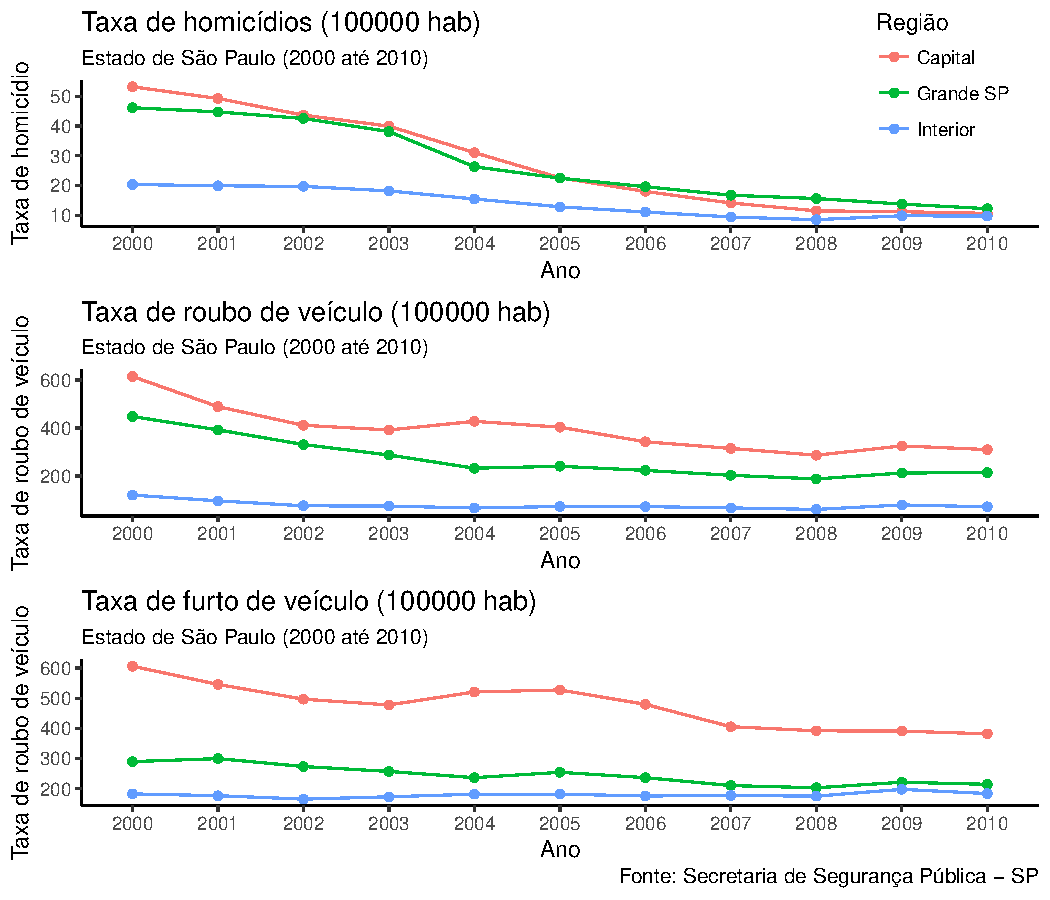
\includegraphics{Análise_1_files/figure-latex/unnamed-chunk-1-1.pdf}

\subsection{Discussão}\label{discussao}

A diferença entre as taxas de crimes entre as cidades do interior do
estado e a capital São Paulo se contrasta com as discussões recentes que
tratam sobre a influência das características locais (ou intra-urbanas)
sobre o crime em uma determinada localidade {[}@glaeser1999there{]}.

\subsection{Referências
Bibliográficas}\label{referencias-bibliograficas}


\end{document}
